\subsection{Bài tập mẫu}

\begin{vd}%[Nguyễn Tấn Linh]%[2H2B1-1]
%	[Đề minh họa BDG 2019-1020] 
	Hình bên là cấu trúc tinh thể muối ăn (NaCl). Các ion $Na^{+}$ và $Cl^{-}$ sắp xếp xen kẽ cách đều nhau theo ba hướng vuông góc với nhau. Biết muối ăn có khối lượng mol là $58,5 \ g/mol$ và khối lượng riêng là $2,2 \ g/cm^{3}$. Khoảng cách giũa hai ion $Na^{+}$ gần nhất trong tinh thể muối ăn là bao nhiêu? Lấy $N_A = 6,02.10^{23} \ mol^{-1}$.
	\begin{center}
		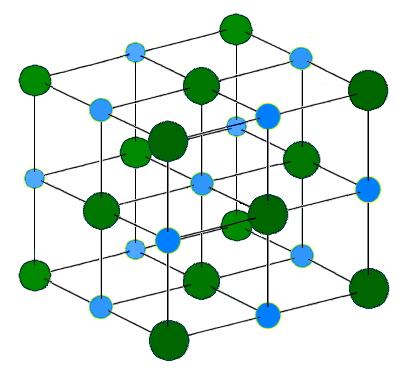
\includegraphics[scale=1.2]{img/Sodium_chloride_crystal.png}
	\end{center}
	\loigiai{
		\begin{phantich}
			Dựa vào mô hình phân tử muối ăn, ta thấy khoảng cách giữa hai ion $Na^{+}$ gần nhất là $d = a\sqrt{2}$, với $a$ là độ dài cạnh của ô cơ sở.
		\end{phantich}
		Nếu không phân biệt ion, thí các ion sắp xếp cách đều nhau.\\
		Thể tích không gian chiếm chỗ của mỗi ion là:  ${V_0} = \dfrac{{{V_m}}}{{2{N_A}}} = \dfrac{M}{{2\rho {N_A}}}$\\
		Mà ${V_0} = {a^3} \to a = \sqrt[3]{{{V_0}}}$\\
		Khoảng cách giữa hai ion gần nhất là $d = a\sqrt 2  = \sqrt[3]{{\dfrac{M}{{2\rho {N_A}}}}}.\sqrt 2  = 3,{97.10^{ - 8}} \ cm$.
	}
\end{vd}

\begin{vd}
	Hình bên là cấu trúc tinh thể caesium clorua (CsCl), ion $Cl^-$ nằm ở tâm của khối lập phương và ion $Cs^+$ nằm ở tám đỉnh của khối lập phương. Biết khối lượng mol của caesium clorua là $168 \ g/mol$, khoảng cách gần nhất giữa hai ion $Cl^-$ là $4.10^{-10} \ m$. Khối lượng riêng của caesium clorua là bao nhiêu? Lấy $N_A = 6,02.10^{23} \ mol^{-1}$.
	\begin{center}
		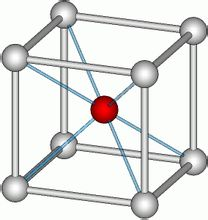
\includegraphics[scale=0.4]{img/8412619e887615d09147c0aadc784128.jpg}
	\end{center}
	\loigiai{
		\begin{phantich}
			Khoảng cách gần nhất giữa hai ion $Cl^-$ là độ dài cạnh $a$ của hình lập phương.\\
			Vì các ion $Cs^+$ sắp xếp đều nhau nên mỗi ion chiếm không gian bằng khối lập phương.
		\end{phantich}
		Thể tích mol là ${{V}_{m}}={{V}_{0}}.{{N}_{A}}={{a}^{3}}.{{N}_{A}}$\\\\
		Khối lượng riêng của $CsCl$ là $\rho =\dfrac{M}{{{V}_{m}}}=\dfrac{M}{{{a}^{3}}.{{N}_{A}}}=4,36 \ g/c{{m}^{3}}$
	}
\end{vd}

\newpage
\begin{vd}
	Biết khí quyển Trái Đất có độ dày nhỏ hơn nhiều so với bán kính $R = 6,4.10^6 \ m$ của Trái Đất, khối lượng mol trung bình là $M = 29 \ g/mol$. Lấy $N_A = 6,02.10^{23} \ mol^{-1}$, áp suất khí quyển ở mặt đất là $p_0 = 10^5 \ Pa$, và gia tốc rơi tự do là $g = 10 \ m/s^2$. Tổng số phân tử trong khí quyển Trái Đất ước lượng là bao nhiêu?
	\loigiai{
		\begin{phantich}
			Áp suất khí quyển là do trọng lực tác dụng lên bề mặt Trái Đất gây ra.\\
			Từ các số liệu đề cho, ta tính được khối lượng khí quyển rồi suy ra được số phân tử.
		\end{phantich}
		Diện tích bề mặt Trái Đất là $S=4\pi {{R}^{2}}$\\
		Khối lượng khí trong khí quyển: ${{p}_{o}}=\dfrac{mg}{S}\to m=\dfrac{4{{p}_{0}}\pi {{R}^{2}}}{g}$\\\\
		Số phân tử trong khí quyển là $N=n{{N}_{A}}=\dfrac{m}{M}{{N}_{A}}=\dfrac{4{{p}_{0}}\pi {{R}^{2}}}{Mg}{{N}_{A}}$\\\\
		Thay số ta được $N = 10^{44}$ phân tử.
	}
	
\end{vd}